\documentclass[12pt,a4paper,oneside,english,brazil]{article}
  \usepackage[abnt-emphasize=bf,abnt-and-type=e,alf]{abntex2cite}
  \usepackage{times}
  \usepackage[left=3cm, top=3cm, right=2cm, bottom=2cm]{geometry}
  \renewcommand{\baselinestretch}{1.5}
  \usepackage{indentfirst}
  \usepackage{graphicx}
  \graphicspath{ {./images/} }
  \renewcommand{\figurename}{\textbf{Fig.}}
  \setlength{\parskip}{0.2cm}

  \usepackage{listingsutf8}
\usepackage{listings}
\usepackage{courier}

\usepackage{xcolor}
\definecolor{lightgray}{rgb}{0.95,0.95,0.95}
\definecolor{codegray}{rgb}{0.5,0.5,0.5}

\lstdefinestyle{meuestilo}{
	inputencoding=utf8/latin1,
  backgroundcolor=\color{lightgray},
	numberstyle=\tiny\color{codegray},
	basicstyle=\ttfamily\footnotesize,
	breakatwhitespace=false,
	breaklines=true,
	captionpos=b,
	keepspaces=true,
	numbers=left,
	numbersep=7pt,
	showspaces=false,
	showstringspaces=false,
	showtabs=false,
	tabsize=2
}

\lstset{style=meuestilo}


    \title{
      \textbf{Hive} \\
      \large um estudo de caso do uso de desenvolvimento guiado por testes para
      alcançar uma arquitetura limpa na construção de um jogo para internet com
      múltiplos competidores
    }
    \author{Hudson Ferreira Leite}
    \date{2021}

\begin{document}
  \maketitle

  % apenas se o número de figuras exceder 10
  \clearpage

    \renewcommand{\listfigurename}{Lista de Figuras}

      \listoffigures

  \clearpage

  \section{Introdução}

    Desenvolver software sempre foi uma atividadade complexa, que pode,
    facilmente,  apresentar desafios das mais diveras naturezas: agendamento;
    má-definição de  requisitos - funcionais ou não; sub - ou super -
    dimensionamento de recursos;não-escalabilidade; etc.

    Negligenciar esse amálgama de possibilidades é um erro comum, e até
    esperado,  de profissionais pouco experimentados, mas, não raro, encontram-se
    exemplarescom bastante quilometragem na carreira.

    O Standish Group demostra, em seu \emph{Chaos Report}
    \cite{ChaosReport2015},  que quanto maior o projeto maior é a chance de
    falha. O mesmo relatório, no entanto, aponta alguns caminhos a seguir para
    encontrar sucesso: \emph{uma arquitetura padrão} e \emph{um processo ágil}.

    Ao mencionar agilidade é possível inferir que a capacidade de adaptação é
    uma  necessidade fundamental para o bom andamento, princípio defendido desde
    a  primeira hora por este tipo de metodologia \cite{ManifestoAgil2001}.

    Quanto à  arquitetura, faz-se evidente que, utilizar um padrão é uma decisão
    que  pode poupar longas, e pouco frutíferas, discursões sobre assuntos já
    consolidados.

  \section{Testes}

    Se estabelecermos um marco na história da programação como sendo a parceiria
    entre a matemática londrina Ada Lovelace, e o, também, matemático londrino
    Charles Babbage\footnote{\cite{Huskey1980}}, pode-se dizer que essa
    disciplina possui mais de 180 anos, e com ela dois grande problemas:

      \begin{itemize}
        \item Especificar o comportamento de um software;
        \item Garantir que um software não possui defeitos.
      \end{itemize}

    No primeiro, por mais avanços que se tenha feito no campo da engenharia de
    software, essa é, ainda, uma área bastante desafiadora. No último, Disjkstra
    estatuiu que \emph{testes mostram a presença, não a ausência de defeitos}
    \cite[p. 16]{Nato1969}.

    Daí a necessidade de se testar \cite[p. xxix-xxx]{Mezaros2007}:

      \begin{itemize}
        \item Paulatinamente construir conhecimento através da retroalimentação
          de hipóteses;
        \item Exaustivamente chegar a um ponto onde não é possível provar a
          presença de defeitos.
      \end{itemize}

    Testes, segundo os métodos tradicionais de desenvolvimento, são feitos em
    etapa posterior a sua construção, para \emph{medir qualidade}. Uma abordagem
    diferente daquela que deseja \emph{construir qualidade}
    \footnote{\cite[p. 7]{FarcicGarcia2015}}. Isso reverbera em \emph{quem} os
    faz: uma equipe diferente da que construiu o software ou o próprio
    desenvolvedor?


    \subsection{Desenvolvimento Guiado por Testes (TDD)?}

      Dentre as práticas que sustentam os métodos ágeis, o uso de testes, como
      uma disciplina de suporte às demais, é um fato consolidado. Mas a
      abordagem, também, conhecida por \emph{testar primeiro} é ainda mais
      difundida nesse  meio.

      Não é raro ver profissionais se referindo a tal técnica como
      "desenvolvimento \emph{orientado a} testes", dando a entender que seu
      objetivo é produzir um código que seja testável, essa é, claramente, uma
      consequência. Ao passo que a tradução que melhor exprime o conceito seria
      "desenvolvimento \emph{guiado por} testes".

      A ideia é extremamente simples \cite[p.1]{FreemanPryce2009}: \emph{escrever um
      teste para um código que ainda não existente}, sumariamente falando, mas
      de maneira mais completa, trata-se de um ciclo de três etapas (Fig.
      \ref{fig:ciclotdd}):

      \begin{center}
        \begin{figure}[h]
          \centering
          \caption{Ciclo TDD}
          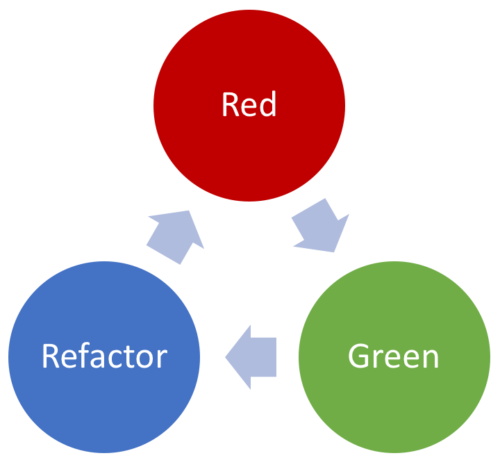
\includegraphics[width=8cm]{ciclo-tdd}
          \label{fig:ciclotdd}
        \end{figure}
        Fonte: Blog da Knowledge21\footnote{\citeonline{Ferreira2018}}
      \end{center}

      \begin{itemize}
        \item Red - Escreva um teste para o qual não existe uma
          implementação, portanto, não deve estar passando nesse
          momento;
        \item Green - Faça passar o teste;
        \item Refactor - Remova duplicações,  melhore a legibilidade.
      \end{itemize}

      Essa postura realoca o papel dos testes, de uma atividade meramente focada
      em descobrir defeitos para uma disciplina centrada na experiência do
      usuário, ao  \emph{guiar} a desenvolvedora no entendimento das reais
      necessidades daqueles, através de um processo dialético de construção de
      conhecimento \footnote{\citeonline[p.28]{Oliveira1992} sugere, ao analisar
      Vygotsky e o processo de formação de conceitos, que os últimos são
      construções culturais, internalizadas pelos indivíduos ao longo do seu
      processo de desenvolvimento.}.

      Daí porque \citeonline[p.3-5]{FreemanPryce2009} posicionam a prática como
      fundamentada em três pilares:
      \begin{enumerate}
        \item Aprendizagem;
        \item Retroalimentação;
        \item Suporte a mudança.
      \end{enumerate}

      

  \section{Arquitetura de Software}

    <texto da sessão>

    \subsection{Arquitetura Limpa}

      <texto da subsessão>

  \section{Como tdd auxilia na busca de uma arquitetura limpa?}

    <texto da sessão>

  \section{O estudo de caso}

    \lstinputlisting{App.js}

  \section{
    O desenvolvimento dos conceitos citados na implementação do estudo de caso
  }

    <texto da sessão>

  \section{Conclusão}

    <texto da sessão>

  \clearpage

  \renewcommand\refname{Referências Bibliográficas}

    \bibliographystyle{abntex2-alf}
    \bibliography{refs}

\end{document}
